\documentclass{article}
\usepackage{float}
\usepackage{graphicx}
\usepackage{geometry}
\usepackage[hidelinks]{hyperref}
\usepackage{cleveref}
\usepackage{indentfirst}
\usepackage{tabularx}
\usepackage{pifont}
\usepackage{url}
\usepackage{matlab-prettifier}
\usepackage[utf8]{inputenc}
\usepackage{upquote}
\usepackage{pifont}
\geometry{hmargin=2.5cm,vmargin=2.5cm}
\hypersetup{
  colorlinks=true, %Colors links instead of ugly boxes
  urlcolor=blue, %Color for external hyperlinks
  linkcolor=blue, %Color of internal links
  citecolor=red %Color of citations
}

\title{\textbf{ModLab}}
\author{Kévin Daigne\\kevin.daigne@hotmail.fr}
\date{Last update of the user guide: September 25, 2024}

\begin{document}

\maketitle

\tableofcontents

\newpage

\section{Overview}

ModLab is a graphical user interface (GUI) developed in MATLAB (and some additional features using shell and batch scripts). It groups together several functionalities needed to manage simulations (text editor, local and remote command prompts, data viewer, etc.). This simplifies simulation processing and enables the different modules to interact with each other. The GUI is made up of several interconnected blocks, as shown in \cref{modlabArch}.

\begin{figure}[H]
\centering
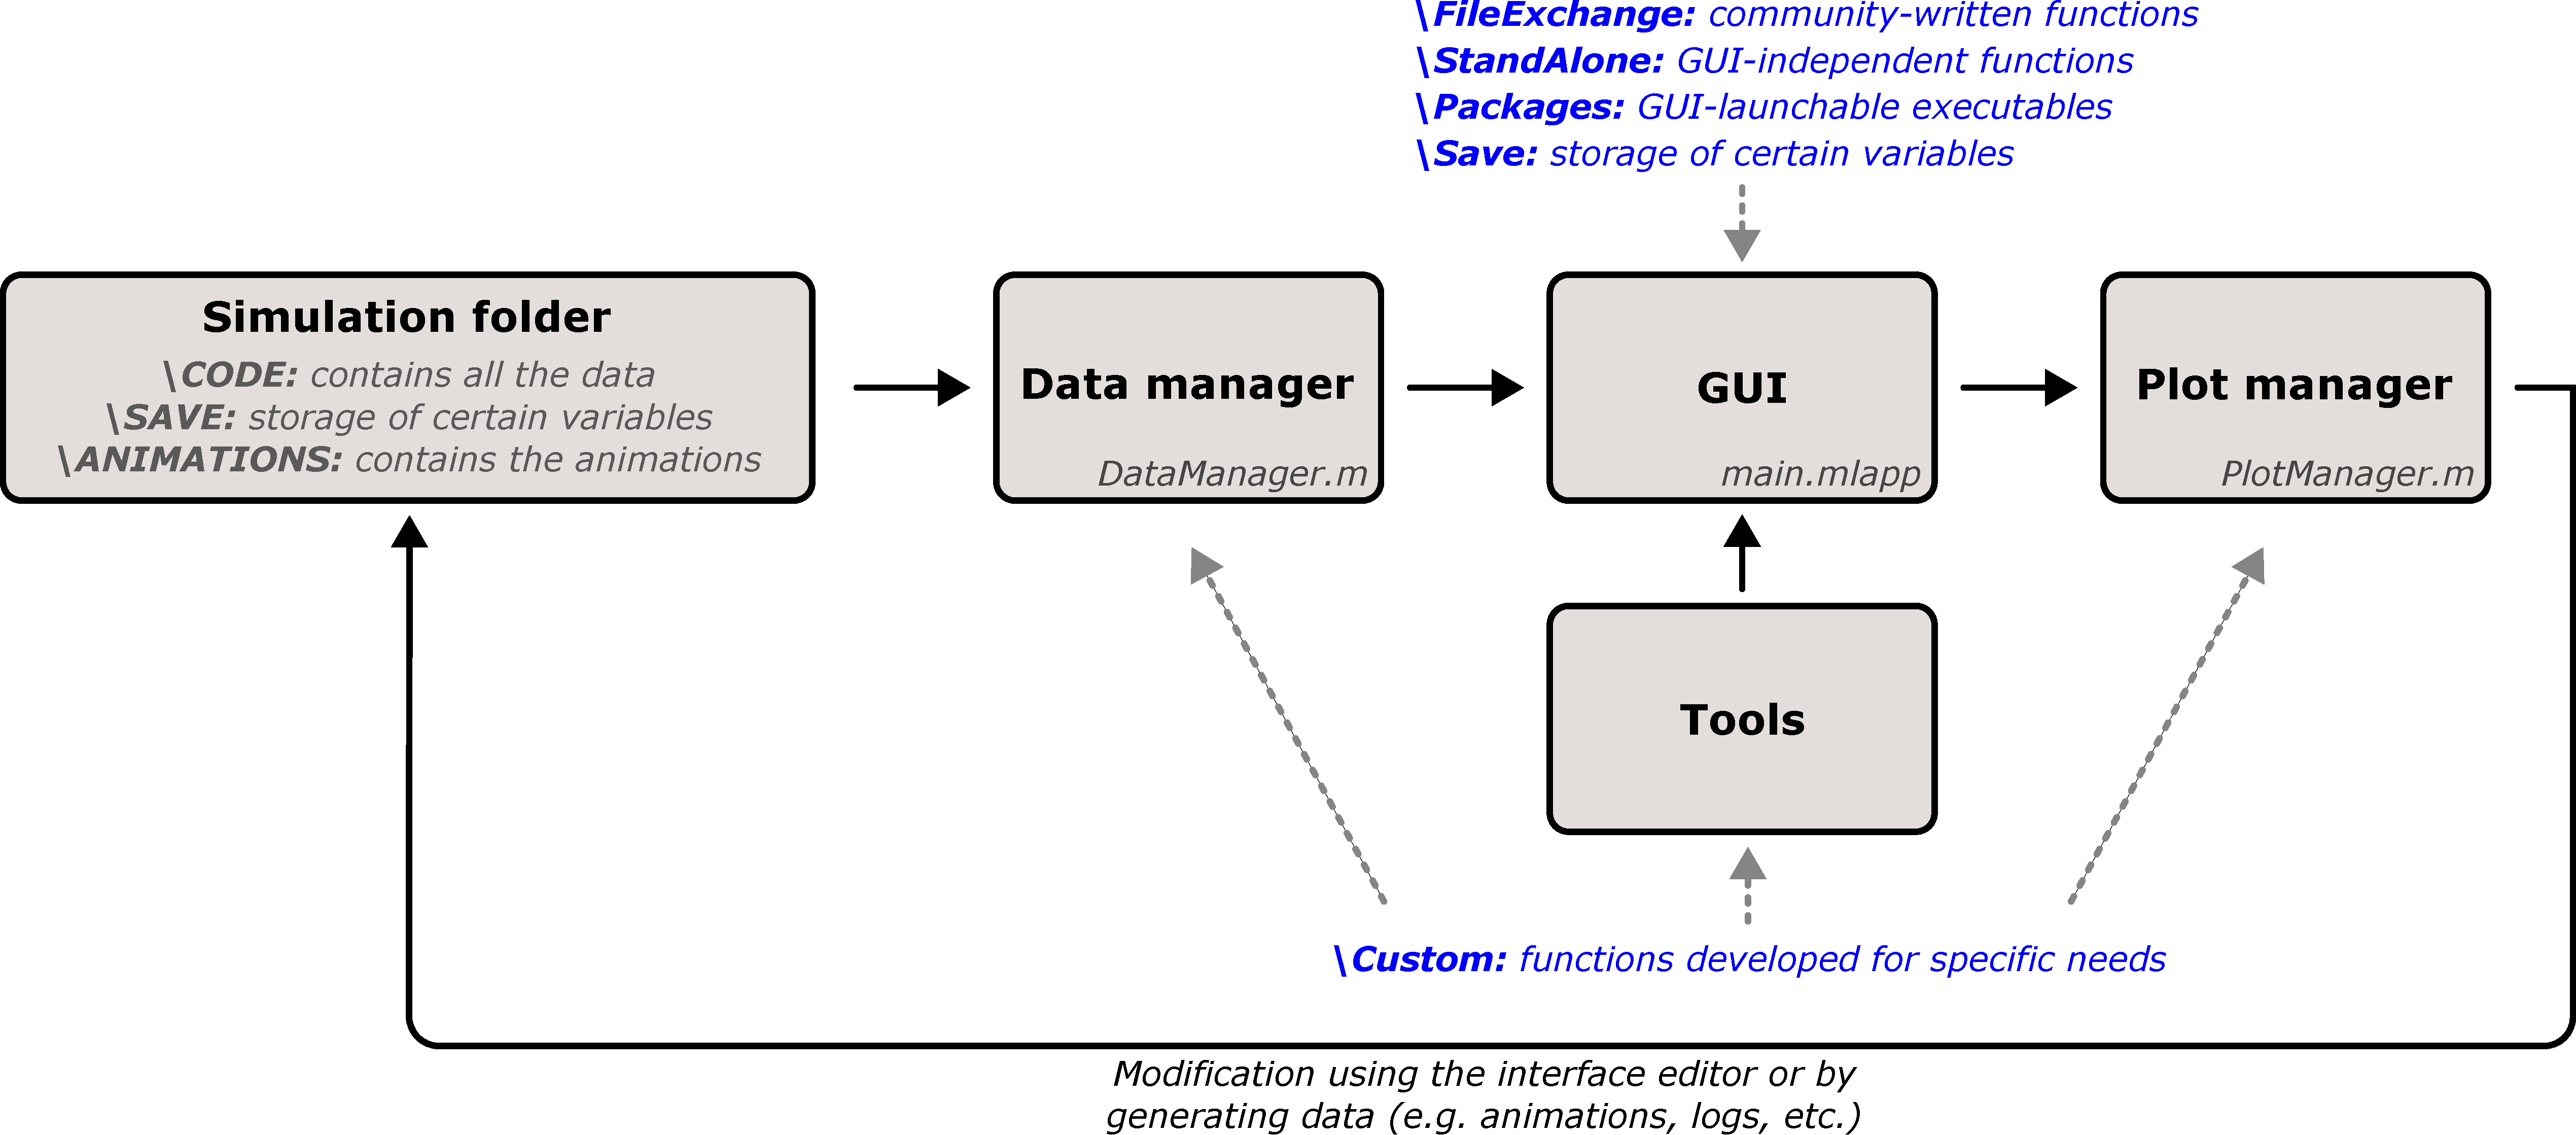
\includegraphics[width=\textwidth]{architecture.pdf}
\caption{ModLab structure}
\label{modlabArch}
\end{figure}

The main purpose of this structure is to bring all the complexity into a single function (main.mlapp) that acts like a black box (which should not be modified except in very specific cases). Thanks to this, the user has almost complete control over processing, by playing with a few inputs and outputs. The main blocks are described below:

\begin{itemize}
    \item \textbf{Simulation folder:} contains all simulation files and others. Data files (model inputs, graphical outputs, etc.) are contained in the \textbackslash CODE subfolder. Only simulation files in this folder can be read. The GUI performs a number of operations, some of which can be stored in the \textbackslash SAVE subfolder. These two subfolders are the main ones, and others can be created according to specific operations (\textbackslash ANIMATIONS, \textbackslash PREPROCESSING, etc.).
    \item \textbf{Data manager:} function to define custom data that can be used within the GUI. This may correspond, for example, to a material parameter contained in a specific file, or to a graphical output on which particular processing is performed.
    \item \textbf{GUI:} function which contains almost all the code defining the GUI. In particular, it includes the definition of objects and their interactions. It uses the MATLAB app designer tool.
    \item \textbf{Plot manager:} all data displayed in the GUI use this function. This provides an easy way of modifying certain properties or data in the graph before it is even created. Combined with the data manager, customized graphs can be defined and displayed directly in two clicks within the GUI.
    \item \textbf{Tools:} user-developed tools, which can interact with all blocks. This provides a simple way of creating functions for specific needs, easily accessible from the GUI, and particularly versatile.
\end{itemize}

There are several subfolders containing functions used by the GUI. In particular, \textbackslash Custom stores all custom functions developed by the user, which can then be called from the data manager, GUI, plot manager and tools.

\section{Prerequisites}

The following components are required:

\begin{itemize}
    \item MATLAB R2024a (with App Designer)
    \item Toolbox: Image Processing Toolbox
    \item Toolbox: Statistics and Machine Learning Toolbox
\end{itemize}

An older version of MATLAB may work, but some features will be inaccessible, leading to errors. To start the GUI, double-click on \path{ModLab.lnk} (the shortcut in the main folder). If it does not work (e.g. for macOS), double-click on \path{\Functions\Management\main.mlapp}.

\section{Simulation folder}

The folder must be selected for all further processing. If the folder is empty, files from another simulation can be imported. In addition, further tabs can be created by clicking on ''+''.

\subsection{\textbackslash CODE}

Contains all simulation files. These files correspond to non-displayable raw data (e.g. model input files) and displayable files (vtk, matrix within a text file, etc.). Only files in this folder can be read by the GUI. The storage of other files (e.g. excel sheets, images, etc.) should be limited, even if possible.

\subsection{\textbackslash SAVE}

Contains all files resulting from GUI computations. For example, it contains all vtk files that have been converted into mat files. This folder is managed by the GUI and is not intended to be modified by the user. Note, however, that if you encounter some issues, deleting the corresponding files in the \textbackslash SAVE folder may solve the problem. Here are a few examples:

\begin{itemize}
    \item Graph based on vtk data is not refreshed: delete corresponding mat files and reload the folder (allowing the Global mat file, which stores the limit, to be refreshed).
    \item Data names are not displayed correctly: reload the folder and, if the problem persists, delete headers\_save.mat. 
    \item Computation speed could not be saved: delete TIME\_save.mat.
\end{itemize}

\subsection{Others}

There are no restrictions on saving other files in the main folder or creating other subfolders.

\subsection{Remote server (cluster)}

\subsubsection{Prerequisites}

There are currently 3 methods available (only one is required for operation).\\

\textbf{PuTTY (Windows)} \newline

You just need to have PuTTY installed on your computer.
\newline

\textbf{sshpass (macOS)} \newline

Follow this procedure (a more detailed procedure can be found on the Internet or by using an AI assistant such as GPT):

\begin{itemize}
    \item  \textbf{Verify Homebrew installation (package management system)}\\
    On terminal:\\
    \verb|brew --version|
    \item \textbf{Install it if it is not}\\
    On terminal:\\ 
    \verb|/bin/bash -c "\$(curl -fsSL https://raw.githubusercontent.com/Homebrew/install/HEAD/install.sh)"|\\
    \verb|echo 'eval "\$(/opt/homebrew/bin/brew shellenv)"' >> ~/.zprofile|\\
    \verb|eval "\$(/opt/homebrew/bin/brew shellenv)"|
    \item  \textbf{Verify sshpass installation}\\
    On terminal:\\
    \verb|sshpass -V|
    \item \textbf{Install it if it is not}\\
    On terminal:\\ 
    \verb|brew install sshpass|
    \item \textbf{Check in which directory it is installed}\\
    On terminal:\\
    \verb|which sshpass|\\
    \item \textbf{Add this path (i.e. previousPath) to system}\\
    On terminal:\\
    \verb|echo 'export PATH="previousPath/sshpass:\$PATH"' >> ~/.zshrc|\\
    \verb|\source ~/.zshrc|
    %\item \textbf{Add this path to MATLAB}\\
    %On MATLAB:\\
    %\verb|setenv('PATH', [getenv('PATH') ':previousPath']);|
\end{itemize}

\textbf{Java (default)} \newline

If none of the above methods are available, use a java-based method (embedded in the GUI, no operation required). However, transfer times are higher. If a key is requested to login, only this method is currently available.

\subsubsection{Format}

For the GUI to recognize that a folder stored on a server corresponds to the local folder, a few rules must be respected. Starting from the specified computation directory on the server, the simulation folder must be contained in the upper folder, no more, no less. Some examples can be found in \cref{simuPath}.

\begin{table}[H]
\centering
\begin{tabularx}{\linewidth}{|l|X|X|}
\hline
& Local & Server \\ \hline
\ding{51}&\path{C:\UpUpFolder\UpFolder\SimuFolder}&\path{CompDir/UpFolder/SimuFolder}\\ \hline
\ding{55}&\path{C:\UpUpFolder\UpFolder\SimuFolder}&\path{CompDir/SimuFolder}\\ \hline
\ding{55}&\path{C:\UpUpFolder\UpFolder\SimuFolder}&\path{CompDir/UpUpFolder/UpFolder/SimuFolder}\\ \hline
\end{tabularx}
\caption{Examples of correct and incorrect simulation paths}
\label{simuPath}
\end{table}

The GUI will automatically add a key of 8 characters (upper and lower case letters) to the name of the simulation folder. For example, SimuFolder will be renamed on the server to SimuFolder\_aBcDeFgH. This helps to identify a computation based on this key. Consequently, if you transfer files manually to the server, you must not use the same key twice. Note, however, that if there is no key, the GUI generates it automatically.

\section{Tools}

\subsection{Use existing tools}

In the tools panel, click on the name to open the readme file (important to avoid any issues) if it exists, and on the checkbox to open or run the tool.

\subsection{Add new tool}

To define a tool, create a folder whose name will define the tool name. Inside, create a MATLAB file, whose name will define the action to follow. Two actions are available (both can be used in the same tool):

\begin{itemize}
    \item mainOpen.m : opens this file when the tool is checked
    \item mainRun.m : runs this file when the tool is checked
\end{itemize}

The content of these functions defines the tool actions. Note that tools can be contained in as many subfolders as required. Only folders containing mainOpen.m or mainRun.m files will be displayed. Moreover, from mainRun.m, you can launch or open as many files as you want. To define a readme.txt, simply place the readme.txt file in the folder containing the mainOpen.m and/or mainRun.m. If several tools use similar functions, consider combining them in the \textbackslash Custom folder.

\section{Text editor}

A text editor is available. Each open file is divided (if applicable) into several sections according to the separator specified in the settings. Each modification is recorded in the log file (particularly useful when modifications are made to the input parameters of a simulation). This editor is not suitable for large files, and a regular text editor should be used in such cases. Note that if you are adding a paragraph to a large document that can be divided into sections, selecting the corresponding section will reduce processing time.

\section{Packages}

\subsection{Use existing packages}

The package (i.e. executable that can be launched from the GUI) can be selected in the settings. A computation is started by clicking on the switch button in the computation panel. If a step is available, it is automatically added as an argument (which can be modified). Currently, only steps from graphics files are detected. Therefore, if only a (non-graphical) data file is available for a step, it will not be taken into account. By default, package is pasted into the simulation folder (inside \textbackslash CODE) and then deleted. This makes it possible to rename the files and obtain a unique name in the task manager, allowing to run several computations in parallel. If this option is disabled, only one computation is allowed. If the computation is stopped outside the GUI, package will not be deleted, and manual deletion in the \textbackslash CODE folder is recommended. Depending on the package, computation can be run locally or on a cluster, according to the selected server.

\subsection{Add new package}

In \textbackslash Packages, create a folder whose name will define the package name. Place the user guide in this folder.  A file is considered as a user guide if it contains user and guide in its name, without being case-sensitive.

\subsubsection{Local}

Create a subfolder named ''Local'' and place all the package in it. The first executable found will be launched.

\subsubsection{Remote server (cluster)}

Create a subfolder named ''Cluster'' and place all the package in it. Set up a launcher for each server, with the following file name: ''Launcher\_serverFormat''. ServerFormat corresponds to the server name in lower case, replacing all special characters by ''\_''. The MATLAB command below can be used to find the launcher name.
\newline\newline
\verb|serverName='example.fr';|\\
\verb|LauncherName=['Launcher_' ...|\\
\verb|lower(replace(serverName,{'[',' ','!','"','#','$','%','&','(',')','*','+',',','-', ...|\\
\verb|'.','/',':',';', ...|\\
\verb|'<','=','>','?','@','\','^','_','`','''','{','}','~',']'},'_'))]|\\
\newline
The result is:\\
\verb|LauncherName = 'Launcher_example_fr'|

\section{Data}

Currently, two types of data are available for reading: those in vtk files, and those in matrix form in text files. The GUI scans all \textbackslash CODE folder and attempts to read all files. Several files can be excluded from this analysis, such as input simulation files, which do not contain raw data. \textbf{If unreadable files are not excluded, this will lead to frequent errors}. Pre-processing, such as naming the data, is stored in headers\_save.mat in \textbackslash SAVE, which can be deleted if necessary. Note that although this is restrictive, each data name must be unique, even if it comes from a different file.

\subsection{Vtk}

The vtk files are particular in the sense that several distinct, sometimes linked (e.g. connectivity and data field), items are stored in a single file. To define limits, it is necessary to read all the file (to find the corresponding data) for all the time steps. To prevent this costly systematic reading, they are first \textbf{converted into mat files} (stored in \textbackslash SAVE). This permits limits to be computed only once, and makes it easier to access each data item, which are now referenced in a structure. This conversion can be carried out in 3 different ways.

\begin{enumerate}
    \item All vtk files in the folder (and more) can be converted using the load tool. In practice, this approach is the most efficient. Significant computation time, but performed at the appropriate moment and avoids forgetting conversion of a few steps.
    \item Each time vtk data is displayed, converts the corresponding file into a mat file. Adds a small but continuous display delay.
    \item If the initialization option is enabled, in addition to the displayed step, converts all previous steps in the same way as described above. Adds a long but rare display delay.
\end{enumerate}

Each file is stored in a mat file with the same name but a different extension (e.g. example\_01.vtk $\rightarrow$ example\_01.mat). The corresponding limits are stored in a single global file for all steps (e.g. example\_01.vtk $\rightarrow$ example\_Global.mat). At each loading, steps not found in \textbackslash CODE are deleted from \textbackslash SAVE. This can be useful for manual processing of step files (i.e. step deletion in vtk or mat format) which, after a new load, will be taken into account, especially in the Global file. This can be used, for example, in the case of a divergence, to remove the unsuitable step.

\subsection{Matrix}

Some files may contain a matrix (several rows of scalars separated by a blank space). For a file containing $N$ rows and $M$ columns, if a name is entered for each column, then the GUI will consider \textbf{$M$ unique data, each one equal to a $N \times 1$ matrix}. If only one name is entered, then the GUI will consider a \textbf{single data equal to a $N \times M$ matrix}. Note that when there is one data item per column, the GUI automatically names the data (which can be modified). In this case, the names may not be explicit, and a tool that gets the names (from a file for example) should be considered.

\section{Display}

\subsection{GUI}

\subsubsection{Default usage}

\textbf{Data format} \newline

\par
When data is selected from the list, \textbf{it is added directly to the equation field}. Each data item is surrounded by square brackets (e.g. [example]). If the data corresponds to a step, the step is added to the name (e.g. [example\%00000]). Note that ''\%'' can be replaced by ''\$'' to be fixed (i.e. not affected by the slider and other buttons). Indices can also be added, in a form that depends on the dimension of the data (e.g. [example\%00000](1:100)). In this case, additional data (explained below) such as the connectivity matrix are automatically recomputed.
\newline

\textbf{Equation}\newline
\par
Each data can be considered as a matrix, and the equation corresponds to the evaluation of these matrices. Consequently, the standard \textbf{rules of matrix algebra apply}. For example, it is possible to add two data if they have the same size, or to compute their square root. Do not forget to use the matrix operator where appropriate, such as ''.*''. The biggest advantage of this approach is that it allows data of different types to be processed together (everything being ultimately matrices). In the case of a plot, a second equation can be added to describe the y-coordinates (sub-equation field). Some examples are given below:

\begin{itemize}
    \item $X_{eq}=$ [stressX\%00000] \& $Y_{eq}=$ empty
    \item $X_{eq}=$ [stressX\%00000]./[stressY\$00000] \& $Y_{eq}=$ empty
    \item $X_{eq}=$ sqrt([stressX\%00000].\^{}2+[stressY\%00000].\^{}2) \& $Y_{eq}=$ empty
    \item $X_{eq}=$ [time] \& $Y_{eq}=$ [height]
    \item $X_{eq}=$ linspace(0,1,numel([height])) \& $Y_{eq}=$ [height]
\end{itemize}

The fact that each data name has to be unique ensures that there is no need for a history and that all the information is contained in the equation. Consequently, an equation can be pasted into another equation field and be read.
\newline

\textbf{Additional data}\newline

\par
Each data can be associated with other, non-displayed data. For example, a connectivity matrix and coordinates can be associated with the selected data. This additional data defines the type of graph that will be displayed, as detailed below:

\begin{enumerate}
    \item \textbf{Surface:} + connectivity and coordinates \textit{(based on $X_{eq}$)}
    \item \textbf{Image with coordinates:} + coordinates \textit{(based on $X_{eq}$)}
    \item \textbf{Image:} none (2D equation) \textit{(based on $X_{eq}$)}
    \item \textbf{Plot:} none (1D equation) \textit{(based on $X_{eq}$ and/or $Y_{eq}$)}
\end{enumerate}

The rule is to use as much additional data as possible. Therefore, if connectivity is found, the graph will be a surface, if only coordinates, an image, etc.
\newline

\textbf{Grounds}\newline

\par
All the comments above can be generalized to \textbf{several grounds} (i.e. different graph types displayed in the same axes). It is possible, for example, to display an image in the background, and add a surface in the foreground. This can be achieved by separating each equation (i.e. ground) \textbf{with ''\#''}. Some examples are given below:

\begin{itemize}
    \item $X_{eq}=$ [velocityField\%00000]\#[stressX\%00000]./[stressY\%00000] \& $Y_{eq}=$ empty
    \item $X_{eq}=$ [stressX\%00000]\#[time] \& 
    $Y_{eq}=$ \#[height] (empty first ground)
\end{itemize}

\subsubsection{Editing}

A graph can be easily edited using the \textbf{PlotManager.m} function. All information is stored in \textbf{info.opts} (axes options) and \textbf{info.grounds} (graph options + data). For instance, this can be used to rotate the graph, apply a coordinate transformation, modify the data field, etc. The possible changes are as numerous as MATLAB capabilities. Other information is also provided in info, such as the current selection in the GUI. To find out about all the possibilities, including the format of the options, take a look at the function \textbf{MultiPlot.m}. In addition, an easy way to understand the format is to use the debug mode and set a breakpoint just before entering in MultiPlot.

\subsubsection{Custom}

Graph editing is mainly relevant for simple and occasional changes. In cases where a change is required regularly, involves multiple data or external data, custom graphs can be used. There are two relatively simple steps to follow:

\begin{enumerate}
    \item In \textbf{DataManager.m}, a graph name is defined, which will then appear in the main list. Associated with this graph, a potential list of elements to be displayed in the sub-list and the data to be loaded. These data can be existing data already available in the GUI, or external data (see the DataManager.m header for more information). The GUI will automatically load the data when you click on the plot button. 
    \item In \textbf{PlotManager.m}, you define all the operations that need to be performed specifically for this graph (see existing examples). Note that even for simple cases (e.g. plot), it is preferable to use the MultiPlot function, which is more efficient and avoids a number of problems. If it does not support the desired graph type (e.g. histogram), then use the usual function.
\end{enumerate}

If the custom graph involves steps, it will be automatically accessible in the animation panel.

\subsection{Animations}

\subsubsection{Single graph}

It works in exactly the same way as described above. The difference is that you cannot modify the equation. Consequently, only raw and custom data can be displayed (the latter is, however, equivalent to editing the equation). Individual animations can be generated for multiple data sets, multiple simulations, multiple formats, etc.

\subsubsection{Current tab}

Animations for multiple graphs work differently. It uses existing graphs from the GUI, modifies them and copies them into the animation figure (whereas single graph animation just involves a modification of an external figure). The main advantage is that it \textbf{preserves any options you may have modified} (e.g. axis names). The disadvantage is that it is a little slower. For the current tab, animations are rarely used, as the format is not particularly suitable. However, there are 2 cases where this can be useful:

\begin{itemize}
    \item Animation for a single graph for which several changes have been made (equation, format, etc.).
    \item Surface-like graph with 3 plots.
\end{itemize}

It should be noted that, even for a single simulation, overview can be used to create animations with side-by-side graphs.

\subsubsection{Overview}

Overview provides an easy way to concatenate \textbf{several graphs from several simulations} into a single figure. Various options are available in the settings. The main ones concern the definition of a common space and data scale (i.e. x and y limits and colormap limits). \textbf{Space scaling} is relatively straightforward: all axes associated with coordinates (surface, image with coordinates, etc.) will have the same limits if desired. \textbf{Data scaling} is a little more tricky. A common scale is defined according to a common word number in labels, either in the colorbar (e.g. surface) or in the x and y axes (e.g. plot). This word number is defined in the settings. See examples below:
\begin{itemize}
\item \textbf{Value=1} (starts from the beginning)\newline
[Force X Contact]$\times$[Force Y Coulomb] $\rightarrow$ [Force]$\times$[Force]\newline
Each axis (or colorbar) which after transformation is called [Force]$\times$[Force] will have the same data range (i.e. limits).
\item \textbf{Value=-1} (starts from the end)\newline
[Force X Contact]$\times$[Force Y Coulomb] $\rightarrow$ [Force X]$\times$[Force Y]
\item \textbf{Value=inf}\newline
Gives a unique data range
\end{itemize}

\end{document}